\documentclass[conference]{IEEEtran} % or [journal]

% --- Essential Packages ---
\usepackage[utf8]{inputenc}
\usepackage[T1]{fontenc}
\usepackage{amsmath}
\usepackage{amssymb}
\usepackage{graphicx}
\usepackage{circuitikz}
\usepackage{booktabs}
\usepackage{subcaption}

% Load these only once
\usepackage{xcolor}                
\usepackage{listings}              

% --- Colors ---
\definecolor{backcolour}{rgb}{0.95,0.95,0.92}
\definecolor{codeblue}{rgb}{0.1,0.1,0.7}
\definecolor{codegray}{rgb}{0.5,0.5,0.5}

% --- Terminal Style Definition ---
\lstdefinestyle{ieee-terminal}{
    language=bash,
    backgroundcolor=\color{backcolour},
    basicstyle=\ttfamily\footnotesize, % Smaller font fits narrow columns better
    keywordstyle=\color{codeblue}\bfseries,
    commentstyle=\color{codegray}\itshape,
    % Box/Frame setup
    frame=single,
    rulecolor=\color{codegray},
    % Margin and spacing fixes for IEEEtran
    linewidth=\columnwidth,   % Keeps box within column limits
    xleftmargin=4pt,          % Indents text away from the left border
    xrightmargin=4pt,         % Indents text away from the right border
    framexleftmargin=4pt,     % Extends the background color to the border
    framexrightmargin=4pt,    % Extends the background color to the border
    breaklines=true,          
    breakatwhitespace=true,
    showstringspaces=false,
    numbers=none,             
    tabsize=2,
    morekeywords={apt,nvim, apt-get, install, update, sudo, git, make, pkg}
}

% --- CRITICAL FIX ---
% This tells LaTeX to use your custom style for all lstlisting blocks globally.
\lstset{style=ieee-terminal}

\usepackage{hyperref}

\hypersetup{
    colorlinks=true,       % Uses colored text instead of ugly default boxes
    linkcolor=codeblue,    % Color for internal links (sections, figures, tables)
    urlcolor=codeblue,     % Color for external web links
    citecolor=codeblue,    % Color for bibliography citations
    pdftitle={Uploading Code to Arduino Using Termux}, % Metadata for the PDF
    pdfauthor={K. Sai Sreevallabh, Shreyas Goud Burra} % Metadata for the PDF
}

% --- Document Info ---
\title{\vspace{1cm}\textbf{Uploading Code Through Termux\\}}
\author{
K. Sai Sreevallabh - EE25BTECH11031\\
Shreyas Goud Burra - EE25BTECH11051
}
\date{}



\begin{document}

\maketitle
% \rule{\linewidth}{0.4pt}

\tableofcontents

\section{Introduction}

Uploading code to Arduino through phone can be done using applications like ArduinoDroid; however uploading solely through Termux is a slightly different because Termux does not have the permissions to directly access the USB port on mobile phones. Hence, this document explains a software workaround to upload code onto an Arduino directly through termux only. 

\section{Overview}

Since Termux cannot directly access the physical USB port on a mobile phone, a native Android application "TCP-UART Transparent Bridge" is employed as a middleware translator, to bypass the strict android permissions. 


\section{Firmware Compilation Using PlatformIO}

PlatformIO is a professional, command-line driven embedded development toolchain that compiles standard C++ code into raw microcontroller firmware.
Ensure that the device on which this is implemented has PlatformIO already installed. 

\subsection{Create a C++ code file}
\begin{lstlisting}
    nvim src/main.cpp
\end{lstlisting}

Type the code that must be uploaded and save the file. \\

\subsection{Generate .hex file:}
\begin{lstlisting}
    pio run 
\end{lstlisting}

The .hex file is now saved in the path
\begin{lstlisting}
    .pio/build/uno/firmware.hex
\end{lstlisting}

The next section explain the working of the core of this approach, TCP-UART Bridge. 

\section{TCP-UART Transparent Bridge}

TCP-UART Transparent Bridge is an app (can be downloaded from Google PlayStore) which acts as a middleware, bridging the gap between Termux and the physical USB port. \\
Since it is a native graphical application, the Android OS grants it the proper, user-approved permissions %via the Android USB Host API
to communicate directly with the Arduino's serial converter.\\
Once USB connection is claimed, the app opens a local Transmission Control Protocol (TCP) network port on the device (e.g. 192.168.0.XXX:8080). \\
Any data that is received over this local network is captured by this app and is injected to the physical USB port. \\
Similarly, any serial data from the Arduino is pushed through the local network, making it possible to replicate the Serial Monitor also. \\


\subsection{Steps}

\begin{itemize}
    \item Once the application is installed from PlayStore, connect the Arduino board to the device using an OTG and click on "connect". 
    \item Grant the USB permissions upon receiving the pop-up.
\end{itemize}

\begin{figure}[h!]
    \centering
    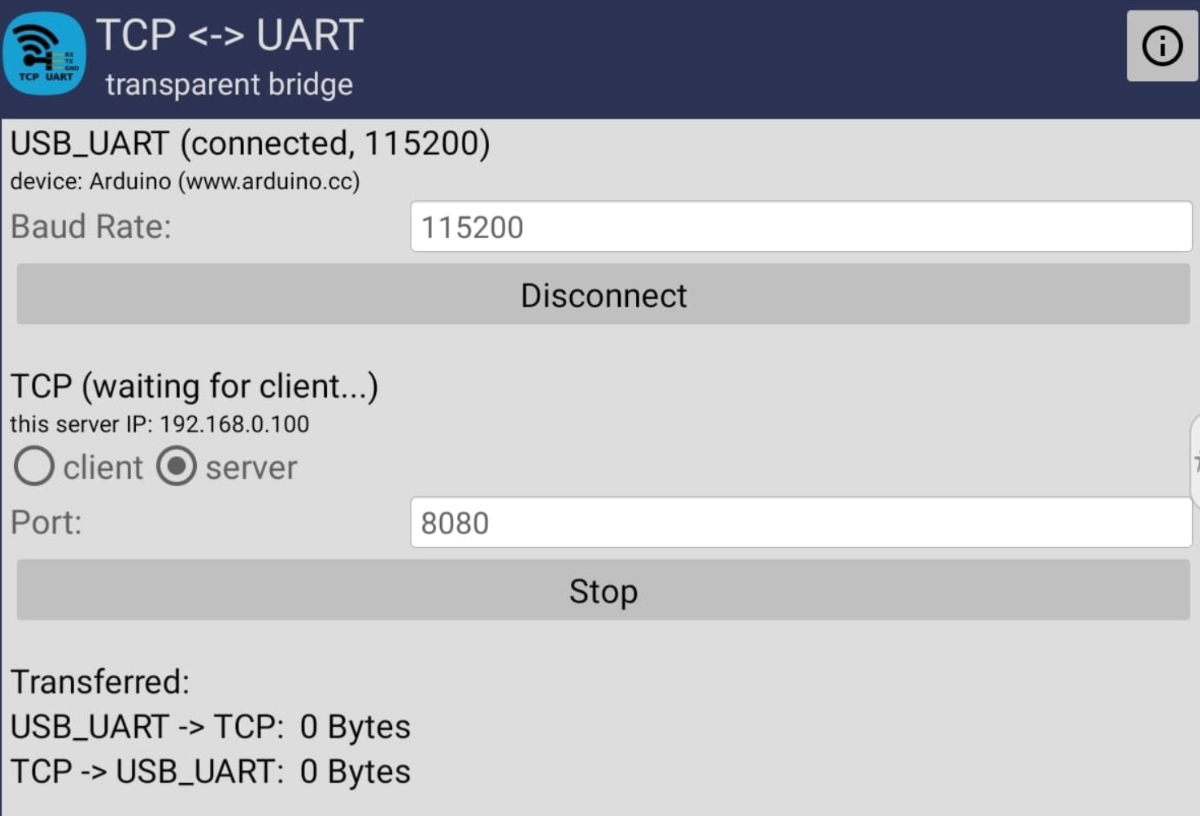
\includegraphics[width=0.7\linewidth]{Figs/tcpuart.png}
    \caption{Interface of TCP-UART Transparent Bridge App}
    \label{fig:placeholder}
\end{figure}

\begin{itemize}
    \item Select the "server" option, under TCP and click start. 
    \item This shows an IP-Address, as shown in the image. 
    \item The IP-Address and Port will be used while uploading the code. 
\end{itemize}

% \begin{figure}[h!]
%     \centering
%     
\includegraphics[width=0.9\linewidth]{tcpuart.png}
%     \caption{Interface of TCP-UART Transparent Bridge App}
%     \label{fig:placeholder}
% \end{figure}
% \newpage
\section{Uploading Using AVRDUDE:}

For installing AVRDUDE
\begin{lstlisting}
    apt install avrdude -y  
\end{lstlisting}

\begin{itemize}
    \item Traditionally, AVRDUDE expects to communicate with a physical hardware end point. 
    \item However, due to restrictions on the Android device, AVRDUDE ability to transfer data over network sockets is leveraged. 
    \item The single command to be used for uploading is listed below. 
\end{itemize}

\begin{lstlisting}
    avrdude -p atmega328p -c arduino -P net:192.168.0.200:8080 -b 115200 -D -U flash:w:.pio/build/uno/firmware.hex
\end{lstlisting}

\begin{itemize}
    \item However, the command must not be executed immediately. (This part is dealt with in the next section). 
    \item The specified IP and Port in the command must perfectly match the server parameters configured in the TCP-UART app. 
    \item By specifying the IPAddress, AVRDUDE treats the firmware upload as standard local network traffic.
    \item This network request is routed to the TCP-UART Android app, which receives the data packets and accurately injects them into the physical USB cable connected to the Arduino.
\end{itemize}

\section{The Timing Issue}

\begin{itemize}
    \item Uploading code onto the Arduino relies on an automatic reset mechanism.
    \item When a device opens a serial connection, it drops the DTR (Data Terminal Ready) line. This causes the a brief pulse on the ATMega328p's RESET pin. 
    \item This immediately reboots it and forces it into the `bootloader', which is a program that listens for a very short time to accept a new .hex file. 
    \item While using the software workaround described above, the DTR line is not brought into the picture i.e. the microcontroller does not auto-reset to listen to the .hex file. 
    \item The manual reset button on the Arduino must be pressed to reset the microcontroller, after which the code uploading command must be executed (i.e. pressing enter after typing the command)
    \item Since the bootloader window is very narrow, timing mismatch causes the AVRDUDE to timeout and upload to fail. 
\end{itemize}

% Uploading code onto the Arduino relies on an automatic reset mechanism. When a device opens a serial connection, it drops the DTR (Data Terminal Ready) line. This causes the a brief pulse on the ATMega328p's RESET pin. This reboots it and forces it into the 'bootloader', which is a program that listens for a very short time to accept a new .hex file. \\

% While using the software workaround discussed above, the DTR line is not brought into the picture i.e. the microcontroller does not auto-reset to listen to the .hex file. 

\section{Hardware Assisted Timing Expansion}

\begin{itemize}
    \item To solve the timing mismatch issue, an electrolytic capacitor ($100\mu F$ to $500\mu F$) is connected between the Arduino's Reset (RES) and Ground (GND) pins, with the negative lead grounded.
    \item The Arduino's reset line has an internal $10k\Omega$ pull-up resistor connected to the 5V supply. Inserting this capacitor creates a Resistor-Capacitor (RC) charging circuit. 
    \item When the physical reset button is held down, the capacitor is instantly discharged, holding the microcontroller at 0V (active reset). 
    \item When the button is released, the capacitor slowly charges through the internal pull-up resistor.  
    \item The voltage at the reset pin over time is determined by the standard RC charging equation:$$V_{reset}(t) = V_{supply} \left(1 - e^{\frac{-t}{RC}}\right)$$.
    \item The microcontroller remains dormant in the reset state until the voltage crosses its internal logic-HIGH threshold (roughly 2.5V to 3.0V).
    \item This physical window (around 1 to 3 seconds) gives the user ample time to comfortably execute the code uploading command before the bootloader times out.
\end{itemize}

% To solve the timing mismatch issue, an electrolytic capacitor (ideally $100\mu F$ to $500\mu F$) is connected between the Arduino's Reset pin (RES) and Ground (GND), ensuring the negative lead is grounded.
% The Arduino's reset line features an internal $10k\Omega$ pull-up resistor connected to the 5V supply. Inserting this capacitor creates a classic Resistor-Capacitor (RC) chargi  ng circuit.
% When the physical reset button is held down, the capacitor is instantly discharged, holding the microcontroller at 0V (active reset). When the button is released, the voltage does not instantly snap back to 5V. Instead, the capacitor must slowly charge through the internal pull-up resistor. 
% The voltage at the reset pin over time is determined by the standard RC charging equation:$$V_{reset}(t) = V_{supply} \left(1 - e^{\frac{-t}{RC}}\right)$$The microcontroller remains dormant in the reset state until the voltage crosses its internal logic-HIGH threshold (roughly 2.5V to 3.0V). This hardware-induced charging delay provides a calculated, physical window (approx. 1 to 3 seconds) that gives the user ample time to comfortably execute the code uploading command before the bootloader times out.


% To solve the timing mismatch issue, a capacitor (around $100\mu F$ to $500\mu F$ is connected between the Reset pin (RES) of the Arduino and the ground, with the negative end of the capacitor connected to the ground.  \\
% The reset pin on the Arduino has a $10k\Omega$ internal pull-up resistor connected to it. Placing the capacitor creates an RC charging circuit. \\
% When the physical reset button is held down, the capacitor is instantly discharged, and the microcontroller is held at 0V (active reset). When the button is released, the voltage does not instantly rise back to 5V. Instead, the capacitor slowly charges through the resistor. Once the voltage of the reset pin is determined by:
% $$V_R = V(1 - e^{\frac{-t}{RC}})$$

% The microcontroller does not exit the reset state until the voltage crosses its internal logic-HIGH threshold (roughly 2.5V to 3.0V). This delay is used to give the user time to execute the code uploading command. 

\section{Serial Monitor}

Once the code is successfully uploaded into the Arduino, Termux can also be used to view the serial data being sent from the Arduino to the device. This is acheived by using Netcat. 

\begin{itemize}
    \item Netcat is used to read and write arbitrary data across network connections using the TCP/IP protocol. 
    \item It perfectly replaces the standard Serial Monitor by connecting directly to the TCP-UART Transparent Bridge app's local server and printing the incoming data to the terminal.
    \item Netcat can be installed using the command
\begin{lstlisting}
    apt install netcat-traditional -y
\end{lstlisting}
    \item To open Netcat and view serial data type the below command
\begin{lstlisting}
    nc 192.168.0.100 8080
\end{lstlisting}
    \item Unlike general Serial monitors, Netcat command does not require the baud rate to be specified because the connection between the terminal and TCP-UART Android app is a local network socket and operates at the maximum network speed. 
    \item The actual hardware baud rate is managed by the TCP-UART Android application.
\end{itemize}


\section{A Step Ahead: Using PlatformIO Only}

\begin{itemize}
    \item In the above method, PlatformIO was used to compile the .hex file, and a separate AVRDUDE command was entered to upload the code, after keeping in mind the timing issues. 
    \item PlatformIO has a native command to directly upload the code i.e. compile the C++ file into a .hex file and upload it to the microcontroller. 
    \item The standard command prompts PlatformIO to search for a physical USB port through which the file can be flashed on the Arduino. However, without access to the physical USB port, the software workaround discussed above is employed and the timing considerations are taken into account. 
    \item For implementing this method, the platoformio.ini file must be altered in order to customise the way in which the uploading is done. 
\end{itemize}

\subsection{Editing the platformio.ini File}

The platformio.ini file acts as the control panel for the uploading process, defining precisely how the code should be compiled and transmitted to the board. \\
By default, Platformio searches for a physical USB port through which the code can be uploaded. To prevent PlatformIO from searching for a physical USB port, add the below line to the platformio.ini file. 

\begin{lstlisting}
    upload_protocol = custom
\end{lstlisting}

\begin{itemize}
    \item Since the default upload method is disabled, an alternate upload command must be specified in the platformio.ini file. 
    \item This command must send the compiled .hex file over to the local network socket. 
    \item Below is the line to add after the upload protocol in the platformio.ini file. 
\end{itemize}
\begin{lstlisting}
upload_command = avrdude -C ~/.platformio/packages/tool-avrdude/avrdude.conf -p atmega328p -c arduino -b 115200 -P net:192.168.0.102:8080 -D -U flash:w:$SOURCE:i
\end{lstlisting}

\begin{itemize}
    \item The IPAddress and Port should be the ones obtained from the TCP-UART Transparent Bridge app. 
\end{itemize}

Save the platformio.ini file. However, there is another minor edit left, which is covered in the next subsection.

\subsection{Delay Script:}

\begin{itemize}
    \item In a standard USB connection, PlatformIO automatically toggles the DTR  line to reboot the Arduino. 
    \item However, while using the software workaround employing the TCP-UART app, this cannot be directly done.  
    \item Hence, the manual reset button must be pressed and released, to reboot the Arduino, keeping in mind the timing considerations. 
    \item The standard command to compile a C++ file and upload the code using PlatformIO outputs multiple lines of dependency checks, build environments, and flash sizing before triggering the actual upload.
    \item Since compilation times vary based on the codebase, the exact time at which the upload begins cannot be discerned. 
 
    \item Hence, a delay script is introduced, which intentionally pauses PlatformIO's upload sequence and display's a visual countdown upto the time the upload begins. 
    \item Create a delay\_script.py file and enter the code provided in 
	    \begin{lstlisting}
	    codes/delay_script.py
	    \end{lstlisting}
\end{itemize}

\subsection{Uploading the Code:}

\begin{itemize}
    \item Open the platformio.ini file once more and add the below line
    \begin{lstlisting}
        extra_scripts = delayScript.py
    \end{lstlisting}
    \item Extra scripts is a parameter in PlatformIO which is used to modify PlatformIO's default behaviour by executing custom Python scripts at defined pre-action or post-action stages of the build environment. 
    \item Make sure that delayScript.py is in the same working directory as the platformio.ini file while using this command; else clearly specify the file path. 
    \item Save and close the platformio.ini file. 
    
    \item Execute the below command to compile and upload the code
    \begin{lstlisting}
        pio run -t upload
    \end{lstlisting}
    \item To manually synchronize the upload, press and hold the manual reset button as soon as the countdown initiates, and release it at around the 2 second mark to allow the bootloader time to initialize before AVRDUDE connects.
    \item Once the upload using PlatformIO is completed, a 'SUCCESS' message is printed in the terminal. 
    \item However, sometimes a 'FAILED' message is printed with an upload error message. In spite of this, if the Writing and Reading are completed upto 100\%, the code has been uploaded completely.
    \item Serial Monitor can be opened in the same way as described in section VIII. 
\end{itemize}

% \subsection{A Note on Intermittent Exit Errors:}
% \begin{itemize}
%     \item The uploading method relies on a TCP-to-USB bridge and hence the timing of the final disconnection is subject to several technicalities of the Android OS and USB. 
%     \item The final disconnection refers to the TCPUART app terminating the temporary session socket assigned to the specific AVRDUDE command. 
%     \item 
% \end{itemize}

\end{document}
